\section{Population improvement versus calibration precision}
\label{sec:block-experiments}

The block hierarchy removes the pair witness's fixed population gap under
the assumptions of Theorem~\ref{thm:block-hierarchy}. It does not imply that
larger blocks always give a more useful certificate at a fixed sample size.
We separate these questions with the exact examples in
Proposition~\ref{prop:block-rare} and all eight finite-support laws in
the supplement's complete finite-support comparison. The laws were examined in the earlier
pairwise comparison; the new protocol freezes the complete block-size grid
and fresh random streams before drawing its observations.

\paragraph{Protocol.}
For every law, 100 independent streams supply nested samples of
$n\in\{256,1024,4096\}$ observations. For each sample, we compare disjoint
blocks of sizes $b\in\{2,4,8,16,32\}$ and the full-sample empirical-minimum
bound in Appendix~\ref{app:erm-comparator}. All methods concern the same
scalar $1$-Lipschitz class. Block calibration uses the sharp target-range
bound $B_b^{\rm blk}$ for $Y\in[-1,1]$ and the KL endpoint in
\eqref{eq:block-lower}. The full-sample comparator uses loss bound four.
Each of the 18 method--sample-size endpoints receives failure probability
$0.05/18$. Their simultaneous statement is per law and repetition; it is
not a joint claim over all 800 streams.

At size two we evaluate the pair formula. Other block scores and the
full-sample comparator use feasible dual lower values. Every one of the
45,579 distinct empirical programs has primal--dual gap at most
$4.01\times10^{-11}$ in empirical-MSE units. Repeated count vectors reuse
the identical optimization result. This finite-support implementation is
not a timing comparison for large continuous representations. All raw
categorical draws, dual certificates, and 14,400 endpoints are retained.

\begin{table}[t]
\centering\small
\caption{Mean lower endpoints at $n=4096$ over all 100 repetitions of each law. $R^*$ is the minimum risk in the same scalar Lipschitz class. Columns $L_b$ use disjoint blocks of size $b$; ERM uses the full sample. A single failure budget $0.05$ per law and repetition covers all six methods and all three sample sizes. The hierarchy orders population witnesses, not these finite-sample endpoints.}
\label{tab:block-hierarchy}
\begin{tabular}{lrrrrrrr}
\toprule
Law & $R^*$ & $L_2$ & $L_4$ & $L_8$ & $L_{16}$ & $L_{32}$ & ERM \\
\midrule
Collapsed binary & 1.0000 & 0.9229 & 0.9355 & 0.9375 & 0.9311 & 0.9159 & 0.9089 \\
Two-atom partial & 0.3315 & 0.2776 & 0.2726 & 0.2573 & 0.2330 & 0.1995 & 0.2755 \\
Three-point V & 0.2222 & 0.1769 & 0.1719 & 0.1589 & 0.1393 & 0.1131 & 0.1763 \\
Five-point zigzag & 0.5400 & 0.3247 & 0.3870 & 0.4203 & 0.4158 & 0.3831 & 0.4697 \\
Partial collapse & 0.2533 & 0.0590 & 0.0964 & 0.1276 & 0.1373 & 0.1244 & 0.2044 \\
Noisy affine & 0.2500 & 0.0678 & 0.1017 & 0.1280 & 0.1352 & 0.1219 & 0.2012 \\
Rare conflict & 0.0250 & 0.0001 & 0.0004 & 0.0007 & 0.0008 & 0.0005 & 0.0116 \\
Affine mismatch & 0.0000 & 0.0000 & 0.0000 & 0.0000 & 0.0000 & 0.0000 & 0.0000 \\
\bottomrule
\end{tabular}
\end{table}


\paragraph{Results and interpretation.}
For partial collapse at $n=4096$, the mean endpoint increases from
$0.0590$ for pairs to $0.1373$ at $b=16$, then decreases to $0.1244$ at
$b=32$. The mean uncalibrated scores continue increasing, from $0.0864$
to $0.2195$ to $0.2370$. The decrease in the endpoint therefore reflects
calibration uncertainty, not a reversal of the population hierarchy.
Full-sample empirical minimization remains stronger on this law, with mean
endpoint $0.2044$. It is also stronger on noisy affine, five-point zigzag,
and rare-conflict laws. Larger blocks are an intermediate statistical and
computational choice, not a uniformly superior replacement for full-sample
optimization.

When the pair witness is already exact, block growth can be unnecessary.
On the partially separated two-atom law, the mean endpoint decreases from
$0.2776$ for pairs to $0.1995$ at $b=32$. By contrast, collapsed binary
noise has a constant population witness but benefits slightly from the
smaller score range and variability of moderate blocks. The affine-mismatch
law remains correctly uninformative for every method because its full
Lipschitz optimum is zero. These different outcomes are all shown in
Table~\ref{tab:block-hierarchy}.

There are no observed simultaneous coverage violations in the 800
law--repetition instances. This is a numerical check against known optima,
not a proof or a replacement for the confidence theorem. The exact curves
in Figure~\ref{fig:block-hierarchy} separately show why block size must
increase to capture sufficiently rare conflicts or noise on many distinct
inputs. Finite-sample block size should be fixed using development evidence,
or selected from a family covered by a joint confidence allocation.

\begin{figure}[t]
\centering
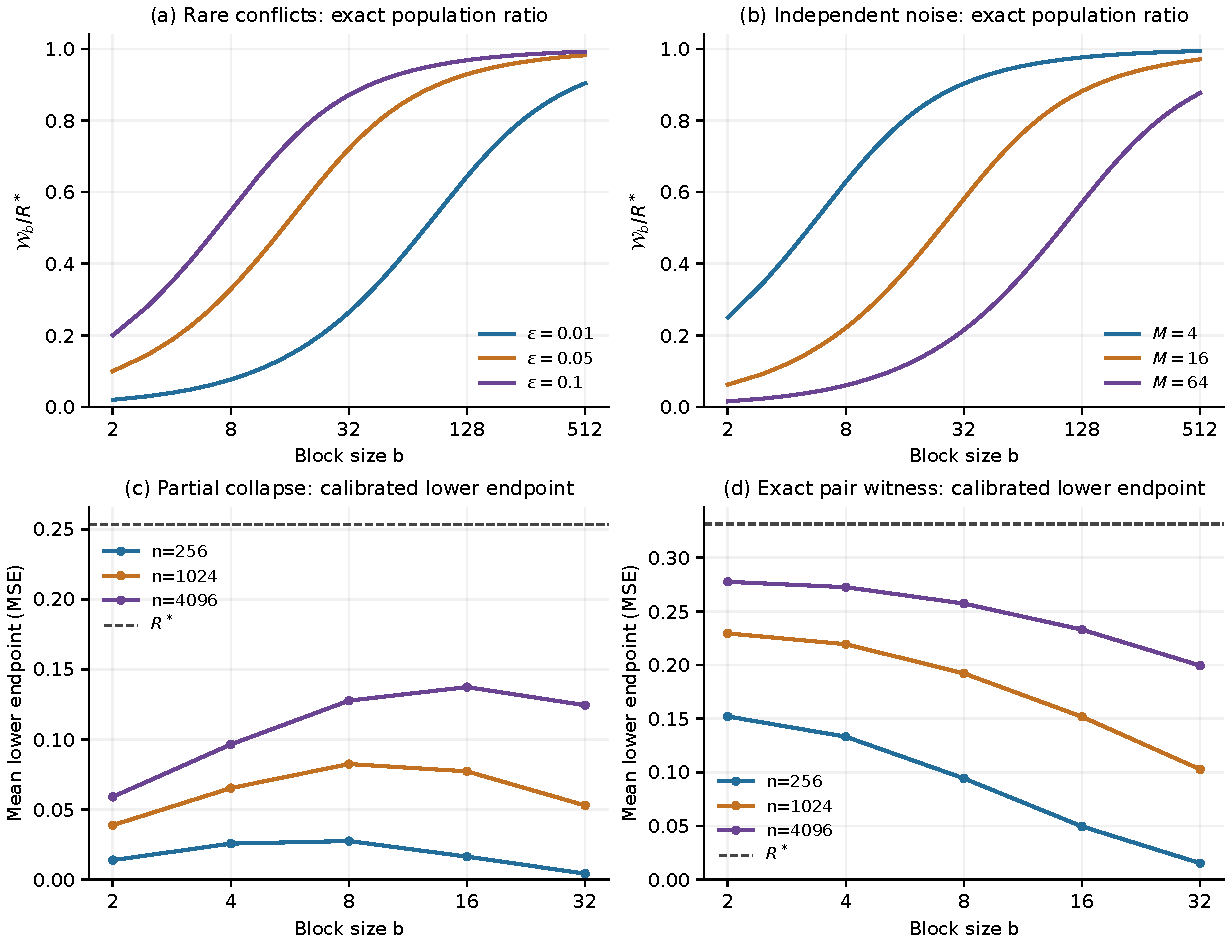
\includegraphics[width=\linewidth]{figures/block_hierarchy.pdf}
\caption{Population and finite-sample effects of block size. Top: exact
ratios from Proposition~\ref{prop:block-rare}, with no Monte Carlo
approximation. Bottom: mean calibrated endpoints over every prescribed
repetition for two contrasting laws; dashed lines are their population
optima. The monotone population hierarchy does not impose monotonicity on
the calibrated endpoints. Table~\ref{tab:block-hierarchy} reports all eight
laws, including cases favoring the full-sample comparator.}
\label{fig:block-hierarchy}
\end{figure}
